\begin{frame}{Experience}

  \begin{columns}
    \begin{column}{0.6\textwidth}
      \begin{itemize}
      \item Since 1.0.0
      \item Scope (by time)
        \begin{itemize}
        \item Bindings (FFI --- foreign function interface)
        \item Analyzers
        \item CLI (TUI) tools for PC and IoT
        \item GUI for fun
        \item Libraries
        \item RE
        \end{itemize}
      \item Nim, Crystal, Zig, Pony
      \end{itemize}
    \end{column}
    \begin{column}{0.45\textwidth}
      \center%
      
\includegraphics[width = \textwidth]{rust_present.png}
    \end{column}
  \end{columns}

  \note{

    \textbf{Начал} более-менее изучать Rust в то время, когда его версия стала
    \textbf{стабильной}, до этого только смотрел примеры кода. В то время
    занимался «железом», поэтому интересно было изучать такие языки, как C, Ada
    (Spark), Rust.

    \textbf{Начинал} с того, с чего обычно не начинают --- с байндингов (FFI)
    для нужных мне инструментов. Затем стал разрабатывать \textbf{анализатор
      НДВ}. Между делом для себя писал консольные тулы (\textbf{слез с Python}).
    Затем помогал в разработке различных библиотек.

    Знаком и писал на других \textbf{новых языках}, также писал и немного знаю
    концепции \textbf{C, Ada, Haskell, Lisp, Python}.

  }
\end{frame}

\begin{frame}{I'm not true programmer}
  \center
  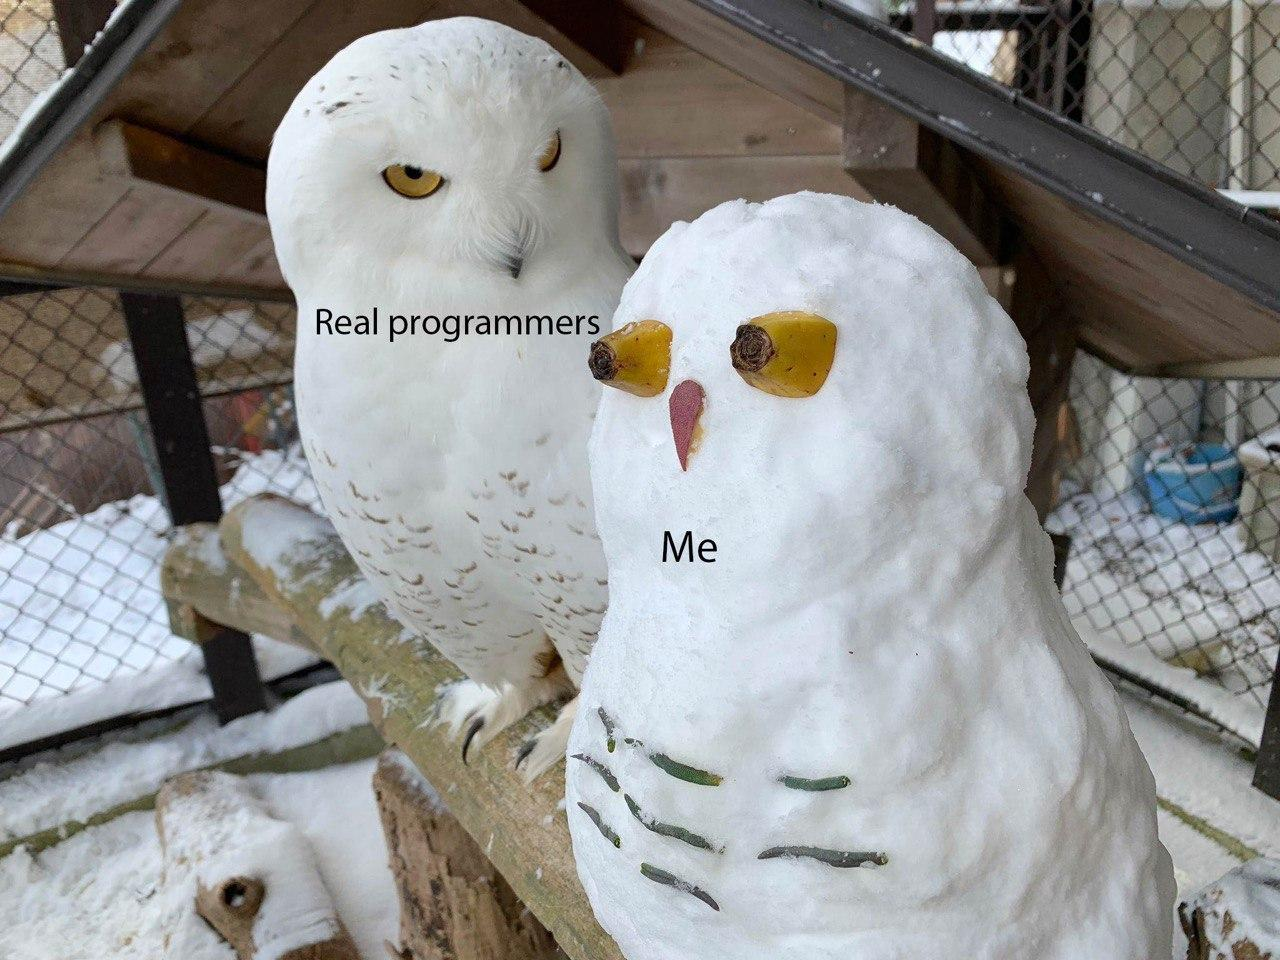
\includegraphics[width = 0.65\textwidth]{real_programmers}

  \note{

    Я не программист и не реверсер. На программиста \textbf{не учился}, читал
    книги, поэтому много \textbf{пробелов в матчасти}.

    Буду рассказывать, исходя только из \textbf{собственного опыта}, моё мнение
    может не совпадать с мнением многих других людей (постоянные холивары,
    некоторые уже вчера смогли убедиться в этом).

    \textbf{Я не буду учить вас Rust}, я просто расскажу основные концепции и
    фишки.

  }
\end{frame}